\subsection{Artificial Intelligense}
Artificial Intelligence (AI) is an umbrella term that encapsulates all algorithms that
show some intelligent behavior.

Machine Learning (ML), a subset of AI [\cref{fig:venn-diagram-ml-deep-learning}], is a system that learns automatically on its own through experiences.
A programmer does not explicitly program it. A ML process makes observations from data to identify possible
patterns that can make future decisions better. Machine Learning aims to allow a system to learn by itself through
experience without any kind of human intervention. Under the hood of many machine learning models are just plain statistics [\cref{fig:venn-diagram-cs-ml-deep-learning}].
The major difference between machine learning and statistics is their purpose.
Statistics is the mathematical study of data.
Machine learning models are designed to make the most accurate predictions.


\begin{figure}[h!]
  \centering
  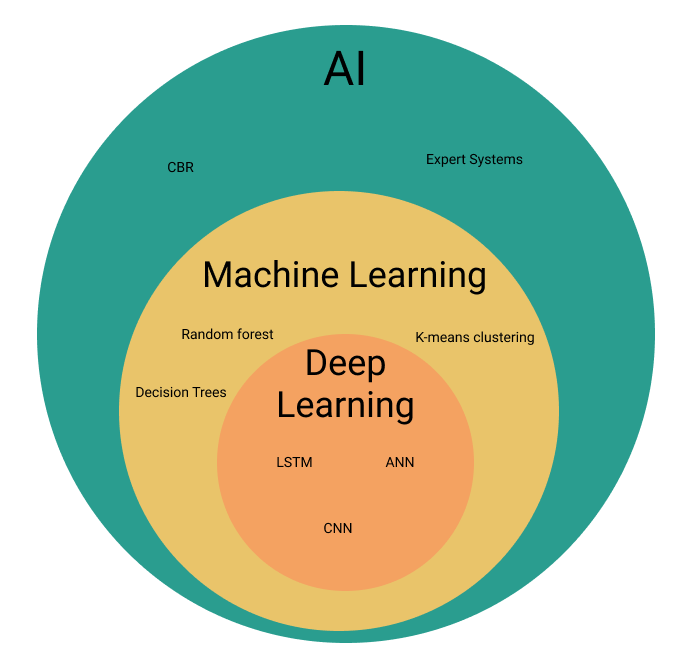
\includegraphics[width=0.5\textwidth]{./figs/illustrations/illustration_venn_diagram_ml_deep_learning.png}
  \hfill
  \caption{Venn diagram of Artificial Intelligense, Machine Learning, and Deep Learning}
  \label{fig:venn-diagram-ml-deep-learning}
\end{figure}
\begin{figure}[h!]
  \centering
  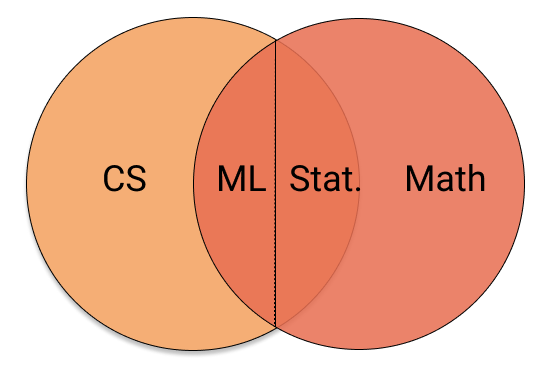
\includegraphics[width=0.5\textwidth]{./figs/illustrations/illustration_venn_diagram_cs_ml_stat_math.png}
  \hfill
  \caption{Venn diagram of Computer Science, Machine Learning, Statistics, and Mathematics}
  \label{fig:venn-diagram-cs-ml-deep-learning}
\end{figure}